\chapter{Experiments: Spotting Anomalies in Patient Visits}
\label{chapter:Experiment}

% what data are used? (period time)
% how to represent the data? (time sequence)
% how to measure the distance? (modified edit distance)

% what preprocess was done? (remove data generated by system)
% Which method to use, why? ( DBSCAN, MM)
	% Can't compute a mean value,	there should be clusters in the data, clustered by department
	% MM is enough. No need to use HMM to complicate the model. Using HMM doesn't explain intuitively, error happened in one phase doesn't lead to error in
	%	the following phase. Different visits don't have direct impact either. Error are usually caused by operators, at least I assume it is this case.
	
This chapter describes the detailed experimental implementation. Following topics will be discussed:
\begin{itemize}
	\item	Which specific data are used? How to represent the data? What preprocess has been done? What related functions are defined?
	\item	Which methods are used? What's the reason to use such methods? 
\end{itemize}
The three topics will be discussed in three sections, respectively. Analysis of the result will be postponed to Chapter~\ref{chapter:evaluation}.

\section{Data Details and Representation}
Since the akseli system has gone through several updation after its first release, many features have changed, including how the visit log is reocrded. Considering this aspect, only data generated after year 2014 is used in the experiment. All the data are from Oulu Hospital, with patient privacy information eliminated. In total, 243K unique visits with 1.93 million entries are retrieved, which spans from January to July. The retrieved data consists of three columns: visit id, event type, and recorded time of the event. Other information, such as which resource generated the data, is not retrieved. Among the retrieved data, 7 event types are adopted. The used event types are: \texttt{ENROLLING}, \texttt{WAITING}, \texttt{IN\_TREATMENT\_ROOM}, \texttt{PAUSED}, \texttt{IN\_TREATMENT\_ROOM\_FROM\_PAUSED}, \texttt{CLOSED}, and \texttt{CANCELLED}.

Huang et al~\cite{huang2012anomaly} proposed to represent the patient visits as a sequence of pairs. Each pair contains the information of (a).~what the event is and (b).~when this event happened. For example, given a sequence showing below
$$
\left\langle(a, 1), (b, 2), (c, 5), (d, 7)\right\rangle 
$$
it means a patient comes to the hospital, and at time 1, the patient encounters event $a$. Then at time 2, the patient encounters event $b$, and so on. The time unit can be selected arbitrarily, such as minutes, hours, or days. Huang et al used days as the time unit. In their work, they tried to cluster the patient traces. However, the patient trace has different length. Thus, typical distance metrics such as euclidean distance is not applicable. To address this problem, they also proposed a new distance metric, based on edit distance.

Edit distance is commonly used in comparing strings and biological sequences, such as proteins. Edit distance is defined as the minimum number of allowd operations used, to transform a string $s$ to another string $t$. For example, if the allowed operations are \textit{delete}, \textit{insert}, and two strings $S$ = \textit{``array''}, $T$ = \textit{``xray''} are given. Then the edit distance between $s$ and $t$ is 3, by taking 3 operations. One potential transformation is: 
\begin{enumerate}
	\item Delete the second letter $r$ in $S$ by $x$. Then $S$ becomes \textit{``aray''}.
	\item Delete the first letter $a$ in $S$. Then $S$ becomes \textit{``ray''}.
	\item Insert letter $x$ at the beginning of $S$. Then $S$ becomes \textit{``xray''}, which is the same with string $T$.
\end{enumerate}

The edit distance problem can be solved effectively by using the dynamic programming technique. Using terminology from dynamic programming, the optimal solution to the edit distance problem can be represented recursively
\begin{equation*}
D(i, j) = \begin{cases} 
   D(i-1, j-1) & \text{if } S\text{[i]} = T\text{[j]} \\
   \min\{D(i-1, j), D(i, j-1)\} + 1       & \text{if } S\text{[i]} \neq T\text{[j]}
  \end{cases}
\end{equation*}

The edit distance only considers the difference between types of events, when applied to the patience visit data. However, the time associated with each event should also makes an effect when comparing two traces. Huang et al addressed this problem by providing a modified edit distance. In the old edit distance, events from two patient trace will either increase the distance by 1 if they belong to different type or 0 if they belong to the same type. In the modified distance, however, the increament caused by two events range from $\left[ 0, 1\right] $ as shown below
%\begin{equation*}
%\delta(\sigma(i), \sigma(j)) = \begin{cases}
%	1 & \text{if} \sigma(i).e \neq \sigma(j).e \\
%	\| \frac{\sigma(i).t - \sigma(j).t}{max\{\sigma(i).t, \sigma(j).t\}} \|	& \text{if) \sigma(i).e = \sigma(j).e
%\end{equation*}

\begin{equation*}
\delta(\sigma_i, \rho_j) = \begin{cases} 
   1 & \text{if } \sigma_i(e) \neq \rho_j(e) \\
   \frac{| \sigma_i(t) - \rho_j(t) | }{max\{\sigma_i(t),~ \rho_j(t)\}}       & \text{if } \sigma_i(e) = \rho_j(e)
  \end{cases}
\end{equation*}
where $\sigma$ and $\rho$ are two patient traces. $\sigma_i$ is the $i$th pair of the trace. $\sigma_i(e)$ and $\sigma_i(t)$ represent the event type and timestamp of the $i$th pair in that trace. The intuition of the above formula is that, if the event types of two pairs in two traces are different, then they contribute 1 to the edit distance. If the event types are the same, then the distance is determined by the timestamp associated with the two events. The closer the timestamps are, the smaller the distance is. 

The modified edit distance seems reasonable. However, some subtle issues exist when the modified edit distance applies to Huang's representation. Consider two patient traces 
\begin{align*}
	&S = \left\langle (a, 1), (b, 1000), (c, 1001), (d, 1002)\right\rangle 	\\
	&T = \left\langle(a, 1), (b, 2), (c, 3), (d, 4)\right\rangle 
\end{align*}
The two traces are very similiar, except that the second pair differs greatly. But this difference propagates further to the third and fourth pairs, incurring more penalty. The modified edit distance will equal almost 3. It would be more reasonable if the distance accounts only the huge different generated in the second pairs, and considers the third and fourth pair the same. To address this problem, in the experiment, a modification on the representation form is applied. Rather than record the absolute timestamp associated with each event, the duration of each event is recorded. Thus, the above two patient traces becomes
\begin{align*}
	&S = \left\langle (a, 1), (b, 999), (c, 1), (d, 1)\right\rangle 	\\
	&T = \left\langle(a, 1), (b, 1), (c, 1), (d, 1)\right\rangle 
\end{align*}
Applying the modified edit distance to the new representation, the answer equals roughly 1, which is more intuitive. Thus, in all experiments, the second representation form is adopted. Minute is used as the time unit.

Another critical point is about preprocessing. After using the second representation form, numerous noise points are observed. It's believed that the noise points are generated by the system itself for logging reasons. The feature of the noise is that all events have a 0 duration time. The noise points consist of approximately 20\% of all data, which incurs great effect in training models. Thus, in the preprocess step, all noise data are manually removed.

\section{Methods}
Chapter~\ref{chapter:clustering} and chapter~\ref{chapter:generative} introduced 4 potential methods. However, only DBSCAN and Markov Chain are used in the experiment. This section explains the reasons for choosing only these two methods and describe related details.

\subsection{Choice of Clustering Method}
As stated in Chapter~\ref{chapter:clustering}, both DBSCAN and K-Means need a elaborate distance metric. This requirement can be fullfilled by using the modified edit distance. Besides this, K-Means also requires efficient computation of the mean value. However, based on the current data representation, it is not clear how to compute the mean. Thus, K-Means is not applicable in this setup. 

One critical phase in applying DBSCAN is how to efficiently compute the $\id{Eps-neighborhood}$.  The DBSCAN algorithm will go through several iterations. Each iteration involves computing $\id{Eps-neighborhood}$ for all points. The efficiency of computing $\id{Eps-neighborhood}$ directly determines the practicability of DBSCAN. A naive implementation is to compute a $N$ by $N$ pair-wise distance table. Then sort the rows in the matrix. After this, finding the $\id{Eps-neighborhood}$ takes only constant time. This process takes $O(N^2)$ space and time. The space complecity can be further reduced to $O(N)$.

A more efficient method, vantage-point tree~\cite{yianilos1993data} can be used in the experiment. Vantage-point tree is a recursively built balanced binary tree. Each non-leaf node consists of two fields, a point functions as a center and a radius, and has two children. The center point is randomly selected from a set of available points. Initially, the set is the whole data points. Then, distances from the center to all the rest points in the set is computed. Next, the radius is set to the median of the distances. After this, the point set is divided into two subsets, one consists of points with a distance shorter than the radius, the other consists of points with a distance longer than the median value. The first set is stored in the left child of current node, and the second set is stored in the right child of the current node. Intuitively, this works as drawing a circle centered on the selected center point. The circle partitions the other points into two parts, with half inside the circle, half outside the circle. This process continues until a leaf node is encountered. This building process takes $O(N \log N)$ time and $O(N \log N)$ space. 

After building the vantage-point tree, finding the $\id{Eps-neighborhood}$ for a single point takes $O(\log N)$ time. Suppose the query point is $p$. Now the query enters a node centered on point $q$ and the radius of the node is $\tau$. Suppose the distance from $p$ to $q$ is $\delta < \tau$. Then the query explores only the left child of $q$ if $\delta + \epsilon \leq \tau$. Otherwise, the right child is also explored. The intuition is that, if one $\id{Eps-neighborhood}$ of query point $p$ is exactly $\epsilon$ far to $p$, then the distance between this neighbour point and the centerd point $q$ is at most $\delta + \epsilon$. If this distance is no larger than the radius associated to the centered node, then there is no need to explore points outside the circle, which reduces the search space by half. As a result, find $\id{Eps-neighborhood}$ for all points takes $O(N \log N)$ time. 

\subsection{Choice of Generative Method}
In the experiment, the simple Markov Chain model is selected for several reasons. Firstly, the patient trace is not long. A typical patient trace has only four events, \texttt{ENROLLING}, \texttt{WAITING}, \texttt{IN\_TREATMENT\_ROOM}, and \texttt{CLOSED}. The longest patient trace doesn't have more than 10 events. Even building an explicit high-order Markov Chain model on these data will still be practical. Another point is that, the type of potential event closely depends on the previous one, rather than depending on an implicit statu. For example, after the event \texttt{ENROLLING}, it is very likely the next event is \texttt{WAITING}. Sometimes, due to special situations such as cancellation of the reservation, the event \texttt{CLOSED} follow. But it is impossible a \texttt{IN\_TREATMENT\_ROOM} event comes, which skips the \texttt{WAITING} phase. The last argument is that, anomaly happened in one phase does not necessarily affect the coming phase. For example, a patient may encounter problems while being in the \texttt{WAITING} phase. But this does not mean the patient may also encounter problems while in \texttt{IN\_TREATMENT\_ROOM} phase. In other words, being in abnormal status in each phase is independent, which is quite contrary to the assumption of HMM that the value of current hidden variable depends on value of the previous hidden variables. As a result, a simple one-order Markov Chain model is selected in the experiment.

In the one-order Markov Chain model, the events are represented using \id{1-of-K} coding schema. Thus, the events are multinomial variables. Another important part of the model is the choice for the emission distribution. Usually, Gaussian distribution is used for modelling continuous variables. However, waiting time is not symmetrically distributed with respect to a mean. The shortest waiting time can only be 0 and the longest waiting time can be very long. The distribution has a skew with a long tail. According to studies in queuing theory, Poisson distribution is more appropriate. Several methods exist to test if Poisson distribution applies, for example, measuring the dispersion. Before stepping into numerical computations, visualizing the distribution is a good start. Related histogram of duration distribution associated with each event is shown in Fig~\ref{fig:fullStat}. Intuitively, the distributions of \texttt{ENROLLING},  \texttt{IN\_TREATMENT\_ROOM}, and \texttt{IN\_TREATMENT\_ROOM\_FROM\_PAUSED} look like Poisson distribution. The distribution of \texttt{WAITING} seems rather different, whcih resembles mixtrue of two Poisson distributions. One plausible explanation is that, these data is obtained from all departments in the hospital. It is possible different departments have different typical waiting time. Luckily, information of department can be also obtained. After extracting data from the largest department, 8915 entries remains. The histogram of these data is shown in Fig~\ref{fig:depStat}. The newly obtained data seems to be more likely from Poisson distribution. Notice that, in these data, only three events remains.


\begin{figure}[!ht]
	\begin{center}
		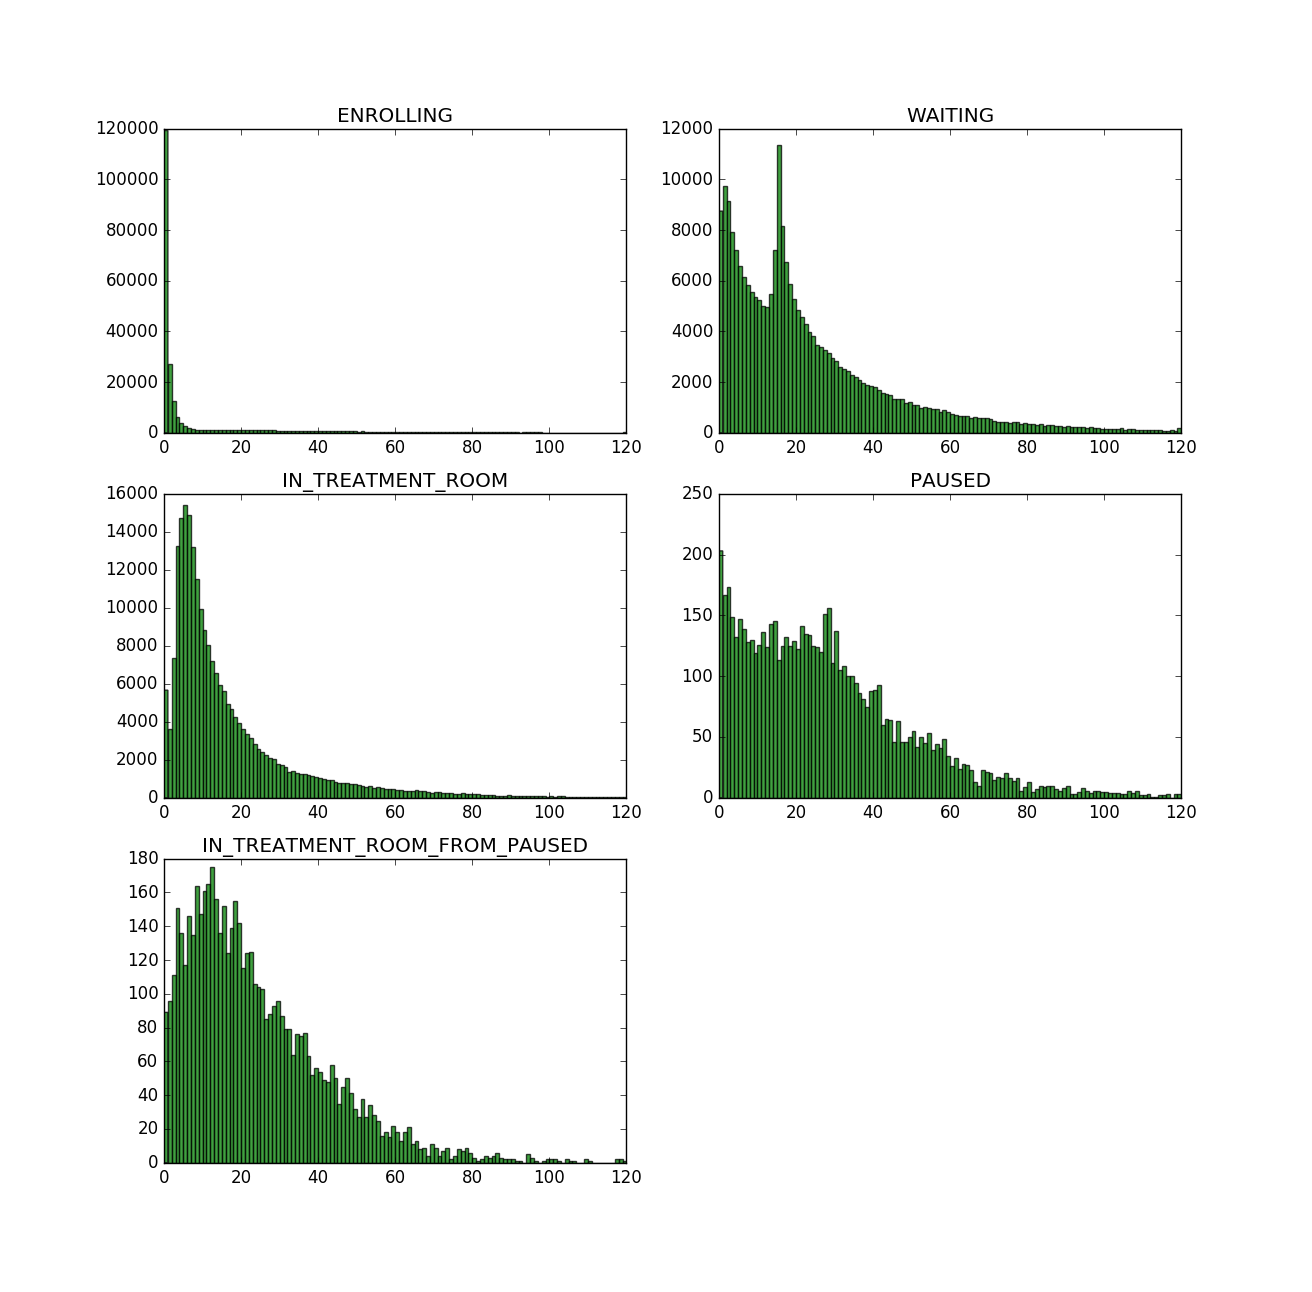
\includegraphics[width=\textwidth]{images/fullStat}
		\caption{Histogram of duration associated with all events}
		\label{fig:fullStat}
	\end{center}
\end{figure}


\begin{figure}[!ht]
	\begin{center}
		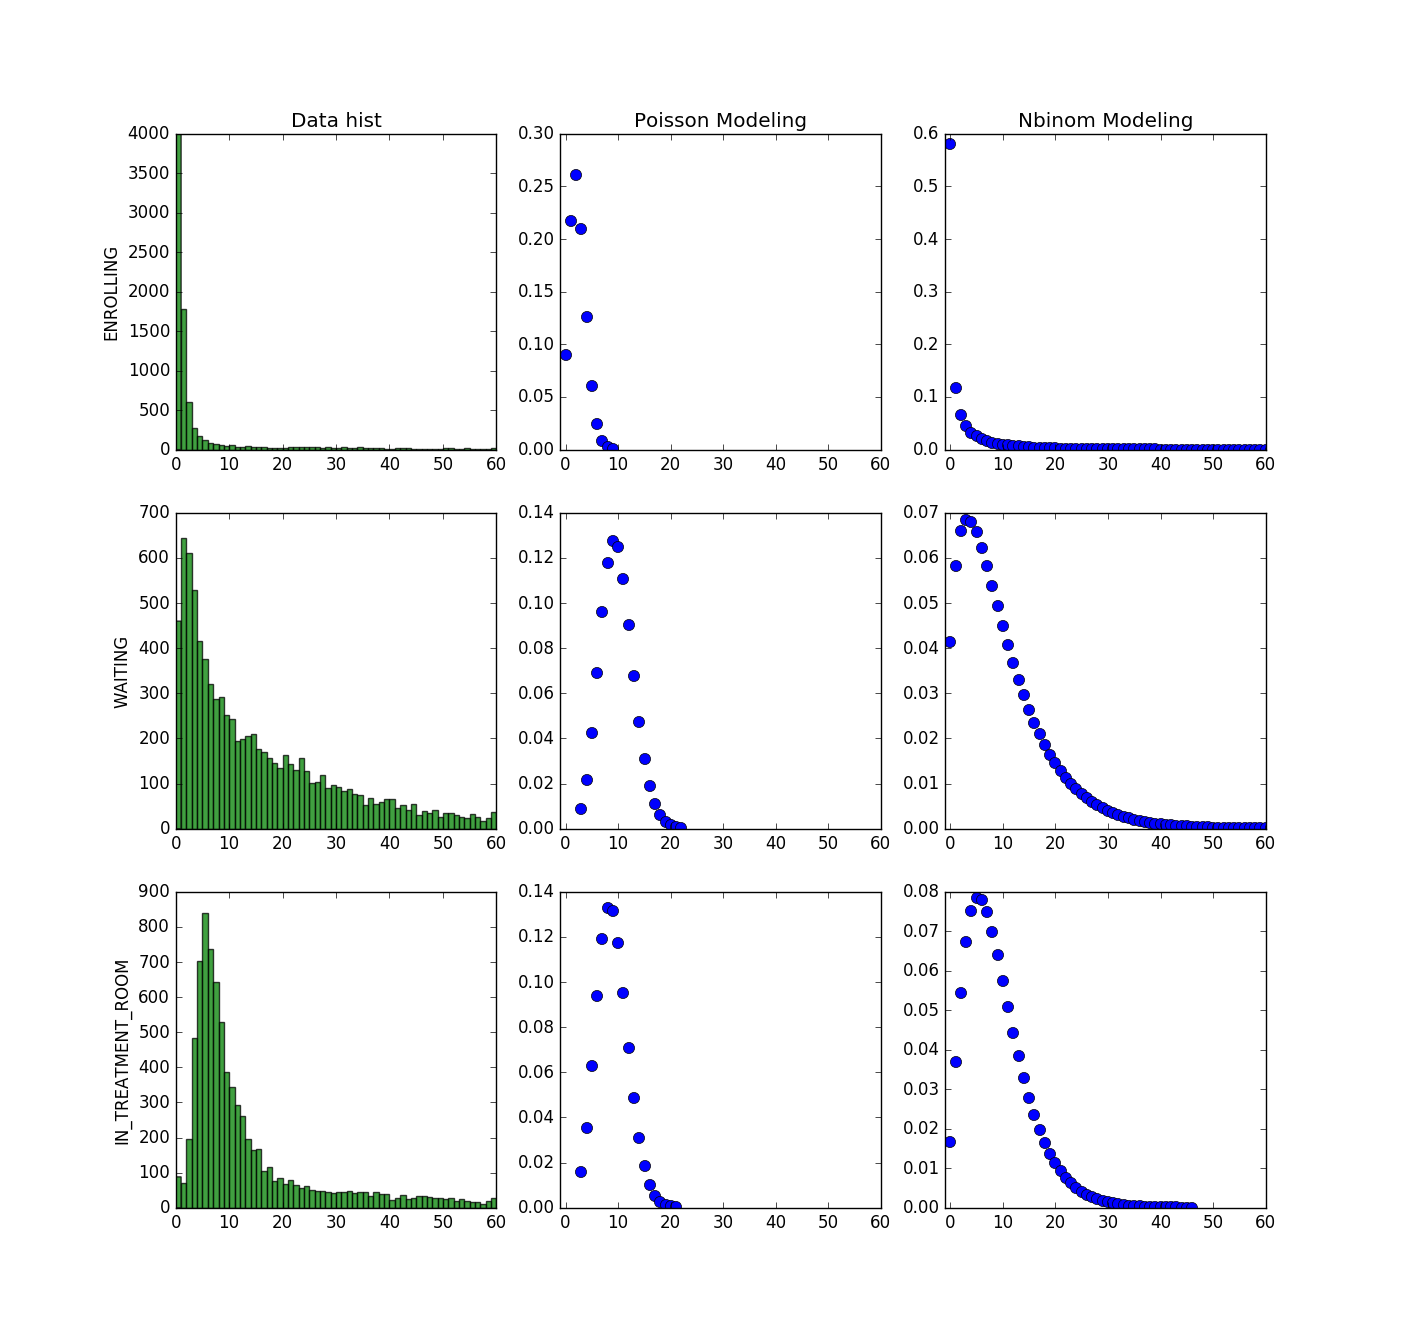
\includegraphics[width=\textwidth]{images/depStat}
		\caption{Histogram of duration associated with all events using data generated by the largest department, together with Poisson distribution fitting and negative binomial distribution fitting.}
		\label{fig:depStat}
	\end{center}
\end{figure}

Next is to compute the dispersion to see if the data distribution really matches Poisson distribution. The formula to compute dispersion is as follow
\begin{equation*}
	D = \frac{\sigma^2}{\mu}
\end{equation*}
where $\sigma^2$ and $\mu$ is the variance and mean value of the data, respectively. One caveat is very large duration time in each distribution. For example, the longest duration in \texttt{WAITING} can be over 1000. Though this situation is very rare, it incurs very large difference when computing $\mu$ and $\sigma$. In fact, such rare values can be considered as the anomalies we are trying to detect. Thus, it makes sense to ignore these cases. It's hard to decide a threshould that determines which part of data should be discarded. In the experiment, the threshould is set to 30. All duration longer than this threshould is not used while computing $\mu$ and $\sigma$. The reason of selecting 30 is that a typical event seldomly lasts more than 30 minutes. In fact, $84\%$ events in this data have less than 30 minutes duration. The computed values are listed in table~\ref{tab:dispersion}
\begin{table}[!ht]
	\begin{center}
		\begin{tabular}{|c|c|c|c|}
			\hline
			events & mean & variance & dispersion \\ \hline
			\texttt{ENROLLING}	& 2.4 & 28.9 & 12.0 \\ \hline
			\texttt{WAITING} & 9.8 & 68.0 & 6.93 \\ \hline
			\texttt{IN\_TREATMENT\_ROOM} & 8.9 & 36.0 & 4.0 \\ 
			\hline
		\end{tabular}
	\end{center}
	\caption{Mean, variance, and dispersion of data generated from largest department.}
	\label{tab:dispersion}
\end{table}
When dispersion equals 1.0, it means the distribution follows Poisson distribution. Typically, data generated from Poisson distribution can have slightly larger dispersion than 1.0. However, as shown in table~\ref{tab:dispersion}, the dispersions are much larger than 1.0. This suggests that the distributions are more likely to come from negative binomial distribution rather than Poisson distribution. Compared to Poisson distribution, negative binomial distribution has ``heavier'' tails and larger variance. Considering this aspect, negative binomial distribution modelling is also implemented in the experiment. The fitting result is shown in Fig~\ref{fig:depStat}. As shown in the figure, negative binomial distribution has a better fitting of the data. Thus, in the final, first-order Markov Chain with negative binomial distribution is chosen as the generative method.
%% The conclusion that nbinom fits better can be numerically verified by using likelihood. But for now, let me just skip this part.
